% Compile with: 
% cd C:\GusDocs\org\thesis\Gus-thesis\internal-defense\
% pdflatex --shell-escape -synctex=1 -interaction=nonstopmode internal-defense.tex 

\documentclass[presentation]{beamer}
%\usepackage[space]{grffile}
\usepackage[utf8]{inputenc}
\usepackage[T1]{fontenc}
\usepackage[normalem]{ulem}
\usepackage{algorithm, algorithmic, amsfonts, amsmath, amssymb, amsthm, amsbsy, array, babel, booktabs, bm, capt-of, circuitikz, color, float, graphicx, grffile, hyperref, lineno, longtable, mathdots, mathptmx, mathtools, minted, pgf, rotating, subfigure, textcomp, tikz, times, units, verbatim, wrapfig, xcolor} % 
\usepackage[outdir=./]{epstopdf}
\usetikzlibrary{shapes, arrows, calc, patterns, decorations.pathmorphing, decorations.markings, positioning}

%newproof, subcaption, 
%\newtheorem{thm}{Theorem}
%\newtheorem{lem}[thm]{Lemma}
%\newproof{pf}{Proof}

\DeclareMathAlphabet\mathbfcal{OMS}{cmsy}{b}{n}

\input{C:/GusDocs/org/texinputs/mystyle-beamer-org}
\titlegraphic{\includegraphics[width=5cm]{C:/GusDocs/org/texinputs/vublogo/RGB/VUB_logo.pdf}}

\renewcommand{\indent}{\hspace*{5em}}
% \useinnertheme{circles}
\setbeamertemplate{itemize items}[circle]
\setbeamertemplate{navigation symbols}{}
\setbeamertemplate{footline}{\hfill \usebeamertemplate***{navigation symbols} \hspace*{0.3cm} \vspace*{0.3cm} \leavevmode \hbox{\begin{beamercolorbox}[wd=0.9\paperwidth,ht=2.25ex,dp=1ex,right]{date in head/foot} \insertframenumber{} \hspace*{1ex} \end{beamercolorbox}} \vskip0pt}
\setbeamerfont{footline}{size=\fontsize{8}{9}}
\addtocounter{framenumber}{0}
\thispagestyle{fancy}
\usetheme{}
\usecolortheme{}

\author{Gustavo Quintana Carapia}
\date{}
\title{Statistical analysis and experimental validation \linebreak of data-driven dynamic measurement methods}

\newcommand\Wider[2][3em]{%
\makebox[\linewidth][c]{%
  \begin{minipage}{\dimexpr\textwidth+#1\relax}
  \raggedright#2
  \end{minipage}%
  }%
}

\begin{document}

\begin{frame}[noframenumbering,plain]
\Wider{\maketitle}
\end{frame}

%\linebreak 

\begin{frame}[label={slide:context}]{A measurement is a dynamic process that \linebreak estimates the input from the sensor response}
\begin{itemize}
\item The sensor is a dynamic system.
\item The sensor response is perturbed with errors.
\end{itemize}
\begin{figure}[htb!]
\centering
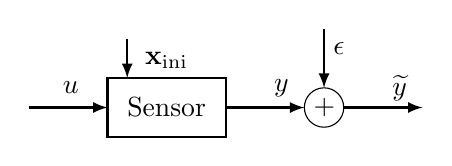
\begin{tikzpicture}[every node/.style={draw,outer sep=0pt,thick}] 
 \node (NB1) [minimum width=1.5cm,minimum height=0.75cm,xshift=0.0cm, yshift=0.0cm] {Sensor};
 \draw [-latex,thick] (NB1.east) ++(0,0) -- +(1.0cm,0);
 \draw [-latex,thick] (NB1.north) ++(-0.5cm,0.5) -- +(0.0cm,-0.5);
 \node[draw=none,fill=none] [above=of NB1,xshift=0.0cm,yshift=-1.0cm] {$\mathbf{x}_{\text{ini}}$};
 \node[draw=none,fill=none] [right=of NB1,xshift=-0.5cm,yshift=0.25cm] {${y}$};
 \node[draw=none,fill=none] [right=of NB1,xshift=1.0cm,yshift=0.25cm] {$\widetilde{y}$};
 \draw [-latex,thick] (NB1.west) +(-1.0,0) -- +(0.0cm,0);
 \node[draw=none,fill=none] [left=of NB1, xshift=0.750cm,yshift=0.25cm] {${u}$}; 
 \draw (2,0.0) circle (2.5mm);
 \node[draw=none,fill=none] [right=of NB1,xshift=0.00mm,yshift=0.0mm]{+};
 \draw [-latex,thick] (NB1.west) +(3.0,0) -- +(4.0cm,0); 
  \draw [-latex,thick] (NB1.west) ++(2.75cm,1.0) -- +(0.0cm,-0.75);
 \node[draw=none,fill=none] [right=of NB1,xshift=0.250cm,yshift=0.75cm] {$\epsilon$};
\end{tikzpicture}
\end{figure}
\begin{itemize}
	\color{blue}
	\item The aim is to assess the uncertainty of \linebreak the data-driven input estimation method.
\end{itemize}
\end{frame}

\begin{frame}[label={slides:have}]{How is the input estimated from the sensor response?}
\begin{itemize}
	\color{blue}
	\item With sensor model
	\begin{itemize}
		\item Kalman filter.
		\item Compensator system.
	\end{itemize}
\end{itemize}
\begin{figure}[htb!]
 \centering
 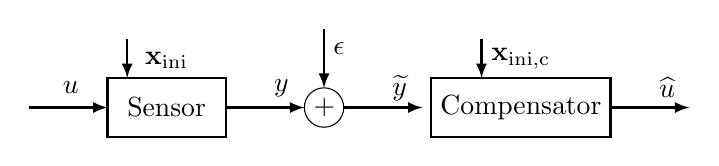
\begin{tikzpicture}[every node/.style={draw,outer sep=0pt,thick}] 
 \node (NB1) [minimum width=1.5cm,minimum height=0.75cm,xshift=0.0cm, yshift=0.0cm] {Sensor};
 \draw [-latex,thick] (NB1.east) ++(0,0) -- +(1.0cm,0);
 \draw [-latex,thick] (NB1.north) ++(-0.5cm,0.5) -- +(0.0cm,-0.5);
 \node[draw=none,fill=none] [above=of NB1,xshift=0.0cm,yshift=-1.0cm] {$\mathbf{x}_{\text{ini}}$};
 \node[draw=none,fill=none] [right=of NB1,xshift=-0.5cm,yshift=0.25cm] {${y}$};
 \node[draw=none,fill=none] [right=of NB1,xshift=1.0cm,yshift=0.25cm] {$\widetilde{y}$};
 \draw [-latex,thick] (NB1.west) +(-1.0,0) -- +(0.0cm,0);
 \node[draw=none,fill=none] [left=of NB1, xshift=0.750cm,yshift=0.25cm] {${u}$};
 \draw (2,0.0) circle (2.5mm);
 \node[draw=none,fill=none] [right=of NB1,xshift=0.00mm,yshift=0.0mm]{+};
 \draw [-latex,thick] (NB1.west) +(3.0,0) -- +(4.0cm,0); 
  \draw [-latex,thick] (NB1.west) ++(2.75cm,1.0) -- +(0.0cm,-0.75);
 \node[draw=none,fill=none] [right=of NB1,xshift=0.250cm,yshift=0.75cm] {$\epsilon$};
 \node (NB2) [minimum width=1.5cm, minimum height=0.75cm, xshift=4.5cm, yshift=0.0cm] {Compensator}; 
 \draw [-latex,thick] (NB2.north) ++(-0.5cm,0.5) -- +(0.0cm,-0.5);
 \node[draw=none,fill=none] [above=of NB2,xshift=0.0cm,yshift=-1.0cm] {$\mathbf{x}_{\text{ini,c}}$};
 \draw [-latex,thick] (NB2.east) ++(0,0) -- +(1.0cm,0);
 \node[draw=none,fill=none] [right=of NB2,xshift=-0.5cm,yshift=0.25cm] {$\widehat{{u}}$};
 \end{tikzpicture}
\end{figure}
\begin{itemize}
	\color{blue}
	\item Without sensor model
	\begin{itemize}
	\item System identification and input estimation.
	\item Optimization.
	\item Data-driven methods.
	\end{itemize}
\end{itemize}
\end{frame}

\begin{frame}[label={slide:have}]{Digital Signal Processors \linebreak offer an alternative to classical approaches}
A DSP, with appropriate algorithms, can 
\begin{itemize}
	\item emulate dynamical systems, or 
	\item implement data-driven methods. 
\end{itemize}
\begin{figure}[htb!]
\centering
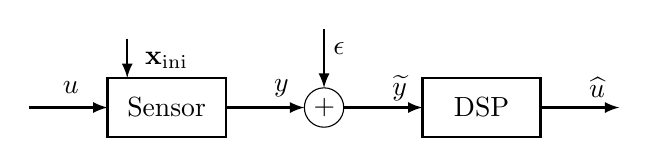
\begin{tikzpicture}[every node/.style={draw,outer sep=0pt,thick}] 
 \node (NB1) [minimum width=1.5cm,minimum height=0.75cm,xshift=0.0cm, yshift=0.0cm] {Sensor};
 \draw [-latex,thick] (NB1.east) ++(0,0) -- +(1.0cm,0);
 \draw [-latex,thick] (NB1.north) ++(-0.5cm,0.5) -- +(0.0cm,-0.5);
 \node[draw=none,fill=none] [above=of NB1,xshift=0.0cm,yshift=-1.0cm] {$\mathbf{x}_{\text{ini}}$};
 \node[draw=none,fill=none] [right=of NB1,xshift=-0.5cm,yshift=0.25cm] {${y}$};
 \node[draw=none,fill=none] [right=of NB1,xshift=1.0cm,yshift=0.25cm] {$\widetilde{y}$};
 \draw [-latex,thick] (NB1.west) +(-1.0,0) -- +(0.0cm,0);
 \node[draw=none,fill=none] [left=of NB1, xshift=0.750cm,yshift=0.25cm] {${u}$};
 \draw (2,0.0) circle (2.5mm);
 \node[draw=none,fill=none] [right=of NB1,xshift=0.00mm,yshift=0.0mm]{+};
 \draw [-latex,thick] (NB1.west) +(3.0,0) -- +(4.0cm,0); 
  \draw [-latex,thick] (NB1.west) ++(2.75cm,1.0) -- +(0.0cm,-0.75);
 \node[draw=none,fill=none] [right=of NB1,xshift=0.250cm,yshift=0.75cm] {$\epsilon$};
\node (NB2) [minimum width=1.5cm, minimum height=0.75cm, xshift=4.0cm, yshift=0.0cm] {DSP}; 
 \draw [-latex,thick] (NB2.east) ++(0,0) -- +(1.0cm,0);
 \node[draw=none,fill=none] [right=of NB2,xshift=-0.5cm,yshift=0.25cm] {$\widehat{{u}}$};
 \end{tikzpicture}
 \end{figure}
 \begin{itemize}
 	\color{blue}
	\item The statistical properties of data-driven methods \linebreak are not straightforward  evident. 
\end{itemize}
\end{frame}

\begin{frame}[label={slides:preview}]{Statistical analysis and experimental validation \linebreak of data-driven dynamic measurement methods}
\begin{itemize}
	\item Formulation of a data-driven step input estimation method.
	\vspace{0.5cm}
	\color{gray}
	\item Thesis contribution.
	\begin{itemize}
		\color{gray}
 		\item Statistical analysis, structured EIV problems.
		\item Experimental validation.
		\item Affine input estimation methods.
 	\end{itemize}
\end{itemize}
\color{black}
\end{frame}

\begin{frame}[label={slide:preliminaries1}]{The input estimation methods are \linebreak formulated as output-error problems}
\begin{figure}[htb!]
\centering
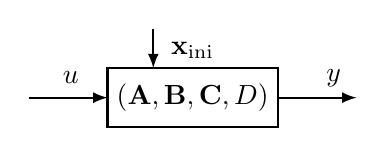
\begin{tikzpicture}[every node/.style={draw,outer sep=0pt,thick}] 
 \node (NB1) [minimum width=1.5cm,minimum height=0.75cm,xshift=0.0cm, yshift=0.0cm] {$\left( \mathbf{A}, \mathbf{B}, \mathbf{C}, D \right)$};
 \draw [-latex,thick] (NB1.east) ++(0,0) -- +(1.0cm,0);
 \draw [-latex,thick] (NB1.north) ++(-0.5cm,0.5) -- +(0.0cm,-0.5);
 \node[draw=none,fill=none] [above=of NB1,xshift=0.0cm,yshift=-1.0cm] {$\mathbf{x}_{\text{ini}}$};
 \node[draw=none,fill=none] [right=of NB1,xshift=-0.5cm,yshift=0.25cm] {${y}$};
 \draw [-latex,thick] (NB1.west) +(-1.0,0) -- +(0.0cm,0);
 \node[draw=none,fill=none] [left=of NB1, xshift=0.750cm,yshift=0.25cm] {${u}$}; 
% \draw (2.3,0.0) circle (2.5mm);
% \node[draw=none,fill=none] [right=of NB1,xshift=1.0cm,yshift=0.25cm] {${y}$};
% \node[draw=none,fill=none] [right=of NB1,xshift=0.00mm,yshift=0.0mm]{+};
% \draw [-latex,thick] (NB1.west) +(3.6,0) -- +(4.6cm,0); 
% \draw [-latex,thick] (NB1.west) ++(3.3cm,1.0) -- +(0.0cm,-0.75);
% \node[draw=none,fill=none] [right=of NB1,xshift=0.250cm,yshift=0.75cm] {$\epsilon$};
\end{tikzpicture}
\end{figure}
\begin{itemize}
	\item With model and exact data, we can write
	\vspace{2mm}
    %\item  With LTI sensor, the measurement dynamics \linebreak can be described using state-space representation: 
\end{itemize}
    %\begin{equation*} \begin{aligned} \mathbf{x}(k+1) &= \mathbf{A} \mathbf{x}(k) + \mathbf{B} {u}(k), \quad \text{with} \quad \mathbf{x}_{\text{ini}} = \mathbf{x}(0) \\ {y}(k) &= \mathbf{C} \mathbf{x}(k) + {D} {u}(k) + {\epsilon}(k) \end{aligned} \end{equation*}
    \begin{equation*} \underbrace{ \begin{bmatrix} y(0) \\ y(1) \\ y(2) \\ \vdots \\ y(N) \end{bmatrix} }_{\mathbf{y}}  = \underbrace{ \begin{bmatrix} \mathbf{C} \\ \mathbf{C} \mathbf{A} \\ \mathbf{C} \mathbf{A}^2 \\ \vdots \\ \mathbf{C} \mathbf{A}^N \end{bmatrix} }_{\mathbfcal{O}} \mathbf{x}(0) + \underbrace{ \begin{bmatrix} \mathbf{D} \\ \mathbf{C} \mathbf{B} & \mathbf{D} \\ \mathbf{C} \mathbf{A} \mathbf{B} & \mathbf{C} \mathbf{B} & \mathbf{D} \\ \vdots & \ddots \\ \mathbf{C} \mathbf{A}^{N-1} \mathbf{B} & \cdots  &  \mathbf{C} \mathbf{A} \mathbf{B} & \mathbf{C} \mathbf{B} & \mathbf{D} \end{bmatrix} }_{\mathbfcal{T}} \underbrace{ \begin{bmatrix} u(0) \\ u(1) \\ u(2) \\ \vdots \\ u(N) \end{bmatrix} }_{\mathbf{u}} \end{equation*}
\end{frame}

\begin{frame}[label={slide:preliminaries3}]{With a step input, the sensor admits an \linebreak augmented autonomous state space representation}
\begin{figure}
\centering
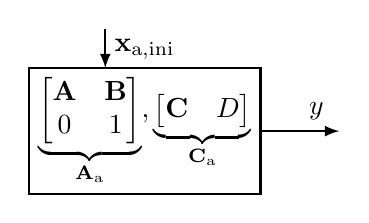
\begin{tikzpicture}[every node/.style={draw,outer sep=0pt,thick}] 
 \node (NB1) [minimum width=1.5cm,minimum height=0.75cm,xshift=0.0cm, yshift=0.0cm] {$ \underbrace{ \begin{bmatrix} \mathbf{A} & \mathbf{B} \\ 0 & 1 \end{bmatrix} }_{\mathbf{A}_\text{a}}, \underbrace{ \begin{bmatrix} \mathbf{C} & D \end{bmatrix} }_{\mathbf{C}_\text{a}} $};
 \draw [-latex,thick] (NB1.east) ++(0,0) -- +(1.0cm,0);
 \draw [-latex,thick] (NB1.north) ++(-0.5cm,0.5) -- +(0.0cm,-0.5);
 \node[draw=none,fill=none] [above=of NB1,xshift=0.0cm,yshift=-1.0cm] {$\mathbf{x}_{\text{a,ini}}$};
 \node[draw=none,fill=none] [right=of NB1,xshift=-0.5cm,yshift=0.25cm] {${y}$};
% \draw [-latex,thick] (NB1.west) +(-1.5,0) -- +(0.0cm,0);
% \node[draw=none,fill=none] [left=of NB1, xshift=0.750cm,yshift=0.25cm] {$u=\bar{u}s$}; 
% \draw (2.7,0.0) circle (2.5mm);
% \node[draw=none,fill=none] [right=of NB1,xshift=1.0cm,yshift=0.25cm] {${y}$};
% \node[draw=none,fill=none] [right=of NB1,xshift=0.00mm,yshift=0.0mm]{+};
% \draw [-latex,thick] (NB1.west) +(4.4,0) -- +(5.4cm,0); 
% \draw [-latex,thick] (NB1.west) ++(4.2cm,1.0) -- +(0.0cm,-0.75);
% \node[draw=none,fill=none] [right=of NB1,xshift=0.250cm,yshift=0.75cm] {$\epsilon$};
\end{tikzpicture}
\end{figure}
\begin{itemize}
	\item Without sensor model, we can estimate first $\mathbfcal{O}_\text{a}$ from
	\vspace{2mm}
   %\item The step input adds a pole at (1,0) to the original system: 
\end{itemize}
  %\begin{equation*} \begin{aligned} \mathbf{x}_\text{a}(k+1) &= \underbrace{ \begin{bmatrix} \mathbf{A} & \mathbf{B} \\ 0 & 1 \end{bmatrix} }_{\mathbf{A}_\text{a}} \mathbf{x}_\text{a}(k) , \quad \text{where} \ \ \mathbf{x}_\text{a}(k) = \begin{bmatrix} \mathbf{x}(k) \\ {u}(k) \end{bmatrix}, \ \ \mathbf{x}_{\text{ini}} = \mathbf{x}(0) \\ {y}(k) &= \underbrace{ \begin{bmatrix} \mathbf{C} & D \end{bmatrix} }_{\mathbf{C}_\text{a}} \mathbf{x}_\text{a}(k) \end{aligned} \end{equation*}
  \small
\begin{equation*} \begin{aligned} & \underbrace{ \begin{bmatrix} y(1) & y(2) & \cdots & y(n) \\ y(2) & y(3) & \cdots & y(n+1) \\ \iddots & \iddots & \iddots \\ y(n) & y(n+1) & \cdots & y(2n-1) \end{bmatrix} }_{ \mathbfcal{H}({y}) } = \underbrace{ \begin{bmatrix} {\mathbf{C}}_\text{a} \\ {\mathbf{C}}_\text{a} {\mathbf{A}}_\text{a} \\ \vdots \\ {\mathbf{C}}_\text{a} {\mathbf{A}}_\text{a}^{n} \end{bmatrix} }_{ {\mathbfcal{O}}_\text{a} }  \underbrace{ \begin{bmatrix} \mathbf{x}_\text{a}(1) & \mathbf{x}_\text{a}(2) & \cdots & \mathbf{x}_\text{a}(n) \end{bmatrix} }_{ \mathbf{X}_\text{ini} } \end{aligned} \end{equation*}
\normalsize
\end{frame}


\begin{frame}[label={slide:preliminaries5}]{After estimating $\widehat{\mathbfcal{O}}_\text{a}$, we can write \linebreak the total response of the system}
\begin{equation*}  {y} = G \ u \ + \ \widehat{\mathbfcal{O}}_\text{a} \ \mathbf{x}_\text{a}(0) , \end{equation*}
\begin{itemize}
\item that is equivalent to
%\begin{equation*}  \underbrace{ \begin{bmatrix}y(0) \\ y(1) \\ \vdots \\ y(T) \end{bmatrix}}_{\mathbf{y}} = \underbrace{ \begin{bmatrix} G & \mathbf{C}_\text{a} \\ G & \mathbf{C}_\text{a} \mathbf{A}_\text{a} \\ \vdots & \vdots \\ G & \mathbf{C}_\text{a} \mathbf{A}_\text{a}^T \end{bmatrix}}_{\mathbf{K}} \begin{bmatrix} \bar{{u}} \\ \mathbf{x}_\text{a}(0) \end{bmatrix} \end{equation*}
\begin{equation*}  \underbrace{ \begin{bmatrix} y(0) \\ \vdots \\ y(N) \end{bmatrix}}_{\mathbf{y}} = \underbrace{ \begin{bmatrix} \mathbf{1}_{N+1} \otimes G & \widehat{\mathbfcal{O}}_\text{a} \end{bmatrix}}_{\mathbf{K}} \begin{bmatrix} u \\ \mathbf{x}_\text{a}(0) \end{bmatrix} \end{equation*}
% \item and admits a least-squares solution
% \begin{equation*}  \begin{bmatrix} \widehat{{u}} \\ \widehat{\mathbf{x}}_{\text{ini}} \end{bmatrix} = \left( \mathbf{K}^\top \mathbf{K} \right)^{-1} \mathbf{K}^\top \mathbf{y} \end{equation*}
\item where $G$ is the sensor static gain.
\end{itemize}
\end{frame}

\begin{frame}[label={slide:preliminaries6}]{To estimate directly the step input,  obtain \linebreak the first difference of the state-space representation} 
\begin{figure}
\centering
\begin{tikzpicture}[every node/.style={draw,outer sep=0pt,thick}] 
 \node (NB1) [minimum width=1.5cm,minimum height=0.75cm,xshift=0.0cm, yshift=0.0cm] {\begin{equation*} \begin{aligned} \Delta \mathbf{x}(k+1) &= \mathbf{A} \Delta \mathbf{x}(k) \\ \Delta {y}(k) &= \mathbf{C} \Delta \mathbf{x}(k) \end{aligned} \end{equation*}};
 \draw [-latex,thick] (NB1.east) ++(0,0) -- +(1.0cm,0);
 \draw [-latex,thick] (NB1.north) ++(-1.5cm,0.5) -- +(0.0cm,-0.5);
 \node[draw=none,fill=none] [above=of NB1,xshift=0.0cm,yshift=-1.0cm] {$\Delta \mathbf{x}_{\text{ini}} = \Delta \mathbf{x}(0)$};
 \node[draw=none,fill=none] [right=of NB1,xshift=-0.5cm,yshift=0.25cm] {$\Delta y$};
% \draw [-latex,thick] (NB1.west) +(-1.5,0) -- +(0.0cm,0);
% \node[draw=none,fill=none] [left=of NB1, xshift=0.750cm,yshift=0.25cm] {$u=\bar{u}s$}; 
% \draw (2.7,0.0) circle (2.5mm);
% \node[draw=none,fill=none] [right=of NB1,xshift=1.0cm,yshift=0.25cm] {${y}$};
% \node[draw=none,fill=none] [right=of NB1,xshift=0.00mm,yshift=0.0mm]{+};
% \draw [-latex,thick] (NB1.west) +(4.4,0) -- +(5.4cm,0); 
% \draw [-latex,thick] (NB1.west) ++(4.2cm,1.0) -- +(0.0cm,-0.75);
% \node[draw=none,fill=none] [right=of NB1,xshift=0.250cm,yshift=0.75cm] {$\epsilon$};
\end{tikzpicture}
\end{figure}
%\begin{equation*} \begin{aligned} \Delta \mathbf{x}(k+1) = \mathbf{A} \Delta \mathbf{x}(k), \quad \Delta {y}(k) = \mathbf{C} \Delta \mathbf{x}(k), \quad \text{with} \quad \Delta \mathbf{x}_{\text{ini}} = \Delta \mathbf{x}(0) \end{aligned} \end{equation*}
where: $\Delta \mathbf{x}(k) = \mathbf{x}(k+1) - \mathbf{x}(k)$ 
\vspace{4mm} 
% \begin{columns}
%  \begin{column}{0.375\columnwidth}
%   where: \linebreak $\Delta \mathbf{x}(k) = \mathbf{x}(k+1) - \mathbf{x}(k)$ 
%   %\newline
%  \end{column}
%   \begin{column}{0.625\columnwidth}
%    If $\Delta {y}$ is persistently exciting of order $L$, \vspace{-4mm} 
%    \[ \text{rank} \left( \mathbfcal{H}_{L+1} \left( \Delta {y} \right) \right) \leq L \] 
%   \end{column}
% \end{columns}
\begin{itemize}
\item If $\Delta {y}$ is persistently exciting enough, the total response is  
\end{itemize}
%\begin{equation*} \mathbf{y} = G \bar{u} + \mathbfcal{H}\left(\Delta {y}\right) \bm{\ell} \end{equation*}
%that is equivalent to
%\begin{equation*} \underbrace{ \begin{bmatrix} y(n+1) \\ \vdots \\ y(T) \end{bmatrix}}_{\mathbf{y}} = \underbrace{ \begin{bmatrix} G & \Delta y(1) & \Delta y(2) & \cdots & \Delta y(n) \\ G & \Delta y(2) & \Delta y(3) & \cdots & \Delta y(n+1) \\ \vdots & \iddots & \iddots & \iddots \\ G & \Delta y(T-n) & \Delta y(T-n+1) & \cdots & \Delta y(T-1) \end{bmatrix}}_{\mathbf{K}} \underbrace{ \begin{bmatrix} \bar{{u}} \\ \bm{\ell} \end{bmatrix} }_{\bm{\theta}} \end{equation*}
\begin{equation*} \underbrace{ \begin{bmatrix} y(n+1) \\ \vdots \\ y(N) \end{bmatrix}}_{\mathbf{y}} = \underbrace{ \begin{bmatrix} \mathbf{1}_{N-n} \otimes G & \mathbfcal{H}\left(\Delta {y}\right) \end{bmatrix}}_{\mathbf{K}} \underbrace{ \begin{bmatrix} u \\ \bm{\ell} \end{bmatrix} }_{\bm{\theta}} \end{equation*}
\end{frame}

\begin{frame}[label={slide:preliminaries7}]{The data-driven step input estimation method converts \linebreak  the output-error into an errors-in-variables problem}
\begin{equation*} \underbrace{ \begin{bmatrix} \widetilde{y}(n+1) \\ \vdots \\ \widetilde{y}(N) \end{bmatrix}}_{\widetilde{\mathbf{y}}} = \underbrace{ \begin{bmatrix} \mathbf{1}_{N-n} \otimes G & \mathbfcal{H}\left(\Delta {\widetilde{y}}\right) \end{bmatrix}}_{\widetilde{\mathbf{K}}} \underbrace{ \begin{bmatrix} u \\ \bm{\ell} \end{bmatrix} }_{\bm{\theta}} \end{equation*}
%and  $\mathbf{E}$ is constructed with the noise data
%\begin{equation*} \mathbf{E} = \begin{bmatrix} 0 & \Delta \epsilon(1) & \Delta \epsilon(2) & \cdots & \Delta \epsilon(n) \\ 0 & \Delta \epsilon(2) & \Delta \epsilon(3) & \cdots & \Delta \epsilon(n+1) \\ \vdots & \vdots & \vdots & & \vdots \\ 0 & \Delta \epsilon(T-n) & \Delta \epsilon(T-n+1) & \cdots & \Delta \epsilon(T-1) \end{bmatrix} \end{equation*}
\begin{itemize}
	\item additive measurement noise $\widetilde{\mathbf{y}} = \mathbf{y} + \bm{\epsilon},$ and $\widetilde{\mathbf{K}} = \mathbf{K} + \mathbf{E}$, 
	\item structured and correlated, 
	\item no evident statistical properties,
	\item hard to get unbiased solution, 
	\item admits a least-squares solution.
\end{itemize}
\end{frame}

\begin{frame}[label={slide:need}]{The data-driven step input estimation \linebreak uncertainty assessment was pending}
This requires to find 
\begin{itemize}
	\item the structured errors-in-variables problem 
	\begin{itemize}
		\item stochastic properties,
	\end{itemize}
	\item the data-driven step input estimation 
	\begin{itemize}
		\item statistical moments, 
		\item mean-squared-error,  
	\end{itemize}
\end{itemize}
\vspace{5mm}
\begin{itemize}
	\color{blue}
	\item The uncertainty assessment
	\begin{itemize}
		\color{blue}
		\item provides confidence bounds w.r.t sample size,
		\item fosters the method utilization in metrology.
	\end{itemize}
\end{itemize}
\end{frame}

\begin{frame}[label={slides:preview}]{Statistical analysis and experimental validation \linebreak of data-driven dynamic measurement methods}
\begin{itemize}
	\color{gray}
	\item Formulation of a data-driven step input estimation method.
	\vspace{0.5cm}
	\color{black}
	\item Thesis contribution.
	\begin{itemize}
 		\item Statistical analysis, structured EIV problems.
		\color{gray}
		\item Experimental validation.
		\item Affine input estimation methods.
 	\end{itemize}
\end{itemize}
\color{black}
\end{frame}


\begin{frame}[label={slide:statistical1}]{To study the least-squares solution of \linebreak an errors-in-variables problem}
\begin{equation*} \widehat{\bm{\theta}} = ( \widetilde{\mathbf{K}}^\top \widetilde{\mathbf{K}} )^{-1} \widetilde{\mathbf{K}}^\top \widetilde{\mathbf{y}} , \end{equation*}
%\vspace{5mm}
where the noise is assumed additive
%\vspace{-2.5mm} 
\begin{equation*} \widehat{\bm{\theta}} = \left( (\mathbf{K}+\mathbf{E})^\top (\mathbf{K}+\mathbf{E})  \right)^{-1} (\mathbf{K}+\mathbf{E})^\top (\mathbf{y}+\bm{\epsilon}) , \end{equation*} 
\vspace{5mm} 
\begin{itemize}
	\color{blue}
	\item I calculated 
	\begin{itemize}
		\color{blue}
		\item the second order Taylor series expansion of $\widehat{\bm{\theta}}$. 
		\item  expressions that predict the bias and covariance,
		\begin{itemize}
			\color{blue}
			\item for unstructured and structured EIV problems.  
		\end{itemize}
	\end{itemize}
\end{itemize}

%\vspace{-2.5mm} 
%\begin{equation*} \begin{aligned} \widehat{\bm{\theta}} &= \big( \mathbf{I} + \underbrace{\mathbf{Q}^{-1} ( \mathbf{K}^\top \mathbf{E} + \mathbf{E}^\top \mathbf{K} + \mathbf{E}^\top \mathbf{E} )}_{\mathbf{M}} \big)^{-1} \big( \underbrace{\mathbf{K}^\top \mathbf{K}}_{\mathbf{Q}} \big)^{-1} (\mathbf{K}+\mathbf{E})^\top (\mathbf{y}+\bm{\epsilon}) \end{aligned}\end{equation*} 
\end{frame}

\begin{frame}[label={slide:statistical8}]{Monte Carlo simulation shows that the expressions for structured EIV  are more susceptible to perturbations}
% \begin{itemize}
% \item The absolute value of the bias and the standard error are proportional to the noise variance and standard deviation.
% \item The bias predictions coincide with the empirical bias, and 
% \item the standard errors are smaller than the estimation bias.
% \end{itemize}
\begin{columns}
\begin{column}{0.35\columnwidth}
\begin{itemize}
	\item Unstructured EIV \linebreak
	\hspace*{-5mm} - uncorrelated, \linebreak
	\hspace*{-5mm} - $\begin{bmatrix} \mathbf{K} &\mathbf{y}\end{bmatrix}$ randomly generated. \linebreak
	\newline
	\item Structured EIV \linebreak
	\hspace*{-5mm} - step input estimation from $2^{\text{nd}}$ order model response. 
\end{itemize}
% \includegraphics[width=1\columnwidth]{./fig/Stat_Fig_4.pdf} 
\end{column}
\begin{column}{0.65\columnwidth}
 \begin{figure}
  \centering
  \includegraphics[width=1\columnwidth]{./fig/Stat_Fig_1u.pdf} 
 \end{figure}
 \begin{figure}
  \centering
  \includegraphics[width=1\columnwidth]{./fig/Stat_Fig_1s.pdf} 
 \end{figure}
\end{column}
\end{columns}
\end{frame}

\begin{frame}[label={slide:statistical10}]{For a $2^{\text{nd}}$ order system, the step input estimation MSE is larger than the CRLB by one order of magnitude}
\begin{figure}
 \centering
 \includegraphics[width=0.65\columnwidth]{./fig/Stat_Fig_3.pdf} 
\end{figure}
\end{frame}

\begin{frame}[label={slides:preview}]{Statistical analysis and experimental validation \linebreak of data-driven dynamic measurement methods}
\begin{itemize}
	\color{gray}
	\item Formulation of a data-driven step input estimation method.
	\vspace{0.5cm}
	\color{black}
	\item Thesis contribution.
	\begin{itemize}
		\color{gray}
		\item Bias and variance analysis, structured EIV problems.
		\color{black}
		\item Experimental validation.
		\color{gray}
		\item Affine input estimation methods.
 	\end{itemize}
\end{itemize}
\end{frame}

\begin{frame}[label={slide:experimental-validation1}]{I designed and built a weighing system \linebreak to collect experimental data from step inputs}
\ctikzset{bipoles/resistor/height=0.075}
\ctikzset{bipoles/resistor/width=0.25}
\begin{figure}[!htb]
\centering
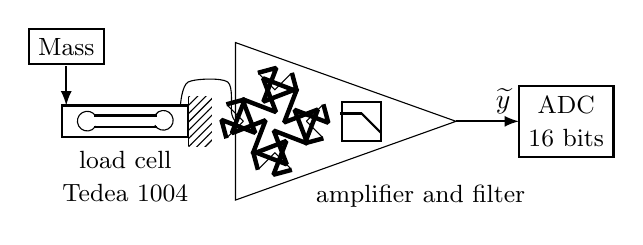
\begin{tikzpicture}[every node/.style={draw,outer sep=0pt,thick}]
\tikzstyle{spring}=[thick,decorate,decoration={zigzag,pre length=0.3cm,post length=0.3cm,segment length=6}]
\tikzstyle{damper}=[thick,decoration={markings,  
  mark connection node=dmp,
  mark=at position 0.5 with 
  {
    \node (dmp) [thick,inner sep=0pt,transform shape,rotate=-90,minimum width=15pt,minimum height=3pt,draw=none] {};
    \draw [thick] ($(dmp.north east)+(2pt,0)$) -- (dmp.south east) -- (dmp.south west) -- ($(dmp.north west)+(2pt,0)$);
    \draw [thick] ($(dmp.north)+(0,-5pt)$) -- ($(dmp.north)+(0,5pt)$);
  }
}, decorate]
\tikzstyle{ground}=[fill,pattern=north east lines,draw=none,minimum width=0.63cm,minimum height=0.3cm]

% load cell
\node (M1) [minimum width=1.6cm,minimum height=0.4cm, xshift=-3cm, yshift=-1cm] {};

\node (ground1) at (M1.east) [ground,yshift=0.0cm,rotate=90,xshift=0.0cm,anchor=north] {};
\draw (ground1.north east) -- (ground1.north west);

\node at (M1.north) [fill=none, xshift=-0.75cm, yshift=0.750cm] (2.0cm, 1.50cm) {\small Mass};
\draw (M1.north) [-latex,thick]  ++(-0.75cm,0.5cm) -- +(0cm,-0.5cm);
\draw (-3.3750cm,-0.935cm) arc(30:330:1.25mm);
\draw (-2.625cm,-1.05cm) arc(210:510:1.25mm);
\draw (M1.west) [thick]  ++(0.4cm, 0.0750cm) -- +(0.80cm,0.0cm);
\draw (M1.west) [thick]  ++(0.4cm,-0.0750cm) -- +(0.80cm,0.0cm);

\node at (M1.south) [align=center, draw=none,fill=none, xshift=0.0cm, yshift=-0.5cm] (2.0cm, 1.50cm) {\small load cell \\ \small Tedea 1004};

% amplifier
\draw (-1.6,-0.0) -- (-1.6,-2.0) -- (1.2,-1) -- cycle;
    \draw (-1.5,-1) to[R] (-1.1,-0.6) to[R] (-0.7,-1);
    \draw (-1.5,-1) to[R] (-1.1,-1.4) to[R] (-0.7,-1);
\draw [-latex,thick]  ++(1.2,-1) -- +(0.8,0);

\node (filter) [minimum width=0.50cm,minimum height=0.50cm, xshift=-0.0cm, yshift=-1cm] {};
\draw [thick]  ++(-0.275,-0.9) -- +(0.275,0.0);
\draw [thick]  ++(0,-0.9) -- +(0.25,-0.250);
\node at (M1.east) [draw=none, fill=none, xshift=4.0cm, yshift=0.25cm] (2.0cm, 1.50cm) {$\widetilde{y}$};
% wire
\draw plot [smooth] coordinates {(-2.3,-0.8) (-2.2,-0.5) (-1.7,-0.5) (-1.65,-0.9) (-1.6,-1)};

\node at (M1.south) [align=center, draw=none,fill=none, xshift=3.75cm, yshift=-0.750cm] (2.0cm, 1.50cm) {\small amplifier and filter};

\node (ADC) [align=center, minimum width=1.2cm,minimum height=0.9cm, xshift=2.6cm, yshift=-1cm] {\small ADC \\ \small 16 bits};
\end{tikzpicture}
\end{figure}
\begin{itemize}
	\item A $5^{\text{th}}$ order sensor model was obtained \linebreak with the sysId toolbox.
\end{itemize}
\end{frame}

\begin{frame}[label={slide:experimental-validation2}]{These are typical step input estimation results \linebreak produced by the data-driven method}
\begin{figure}[htb!]
\centering
\hspace*{-5mm} \includegraphics[width=1.1\columnwidth]{./fig/Exp_Fig_1.pdf} 
\end{figure}
\begin{columns}
\begin{column}{0.5\columnwidth}
Processing a $5^{\text{th}}$ order \linebreak model response.
\end{column}
\begin{column}{0.5\columnwidth}
Processing a measured \linebreak sensor response.
\end{column}
\end{columns}
\end{frame}

\begin{frame}[label={slide:experimental-validation3}]{Monte Carlo simulation shows that, for SNR > 40 dB \linebreak the bias and variance are well predicted}
\begin{figure}
 \centering
 \includegraphics[width=0.65\columnwidth]{./fig/Exp_Fig_2.pdf} 
\end{figure}
\begin{figure}
 \centering
 \includegraphics[width=0.65\columnwidth]{./fig/Exp_Fig_3.pdf} 
\end{figure}
\begin{itemize}
	\color{blue}
	\item The data-driven step input estimation MSE is at most \linebreak one order of magnitude larger than the EIV problem CRLB.
\end{itemize}
\end{frame}

\begin{frame}[label={slide:experimental-validation6}]{There are periodic components \linebreak in the measurement noise}
\begin{figure}
\centering
\includegraphics[width=0.65\columnwidth]{./fig/Exp_Fig_7.pdf} 
\end{figure}
\begin{figure}
\centering 
\includegraphics[width=0.65\columnwidth]{./fig/Exp_Fig_9.pdf} 
\end{figure}
\begin{itemize}
	\color{blue}
	\item Considering the residuals, \linebreak the SNR was adjusted from 55 dB to 50 dB. 
\end{itemize}
\end{frame}

\begin{frame}[label={slide:experimental-validation5}]{After processing 100 measured responses, \linebreak the bias and variance decrease w.r.t. sample size} 
% \begin{figure}
%  \centering
%  \includegraphics[width=0.6\columnwidth]{./fig/Exp_Fig_8.pdf} 
% \end{figure}
\begin{figure}
 \centering
 \includegraphics[width=0.65\columnwidth]{./fig/Exp_Fig_11.pdf} 
\end{figure}
% \begin{itemize}
% 	\color{blue}
% 	\item The step input estimation method is useful \linebreak when the measurement noise is not Gaussian white. 
% \end{itemize}
\end{frame}

\begin{frame}[label={slide:experimental-validation4}]{The estimation MSE is smallest \linebreak for orders larger than the true order}
\begin{figure}
  \centering
  \includegraphics[width=0.65\columnwidth]{./fig/Exp_Fig_4.pdf} 
\end{figure}
\begin{itemize}
$10^4$ simulated responses from $5^{\text{th}}$ order model.
\end{itemize}
\end{frame}

% \begin{frame}[label={slide:experimental-validation8}]{Observations of the experimental validation of the step input estimation method}
% \begin{itemize}
% \item In simulation, the input estimation MSE is close to the CRLB theoretical minimum for biased estimators.
% \item The step input estimation method is useful in practical applications where the whiteness assumption of the measurement noise is not fulfilled. 
% \item The noise variance obtained from the sensor steady state response underestimates the measurement noise variance.
% \item Using the predictions, the uncertainty assessment is provided for given sample size and noise variance.
% \end{itemize}
% \end{frame}

\begin{frame}[label={slides:preview}]{Statistical analysis and experimental validation \linebreak of data-driven dynamic measurement methods}
\begin{itemize}
	\color{gray}
	\item Formulation of a data-driven step input estimation method.
	\vspace{0.5cm}
	\item Thesis contribution.
	\begin{itemize}
 		\color{gray}
 		\item Statistical analysis, structured EIV problems.
		\item Experimental validation.
		\color{black}
		\item Affine input estimation methods.
 	\end{itemize}
\end{itemize}
\color{black}
\end{frame}

\begin{frame}[label={slide:affine-input-estimation1}]{Can we estimate affine inputs \linebreak with a data-driven method?}
\begin{figure}
\centering
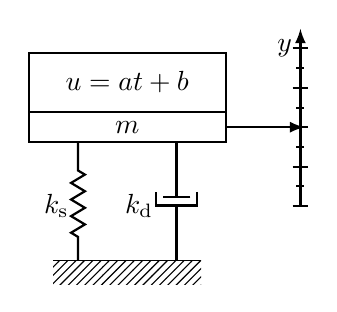
\begin{tikzpicture}[every node/.style={draw,outer sep=0pt,thick}]
\tikzstyle{spring}=[thick,decorate,decoration={zigzag,pre length=0.3cm,post length=0.3cm,segment length=6}]
\tikzstyle{damper}=[thick,decoration={markings,  
  mark connection node=dmp,
  mark=at position 0.5 with 
  {
    \node (dmp) [thick,inner sep=0pt,transform shape,rotate=-90,minimum width=15pt,minimum height=3pt,draw=none] {};
    \draw [thick] ($(dmp.north east)+(2pt,0)$) -- (dmp.south east) -- (dmp.south west) -- ($(dmp.north west)+(2pt,0)$);
    \draw [thick] ($(dmp.north)+(0,-5pt)$) -- ($(dmp.north)+(0,5pt)$);
  }
}, decorate]
\tikzstyle{ground}=[fill,pattern=north east lines,draw=none,minimum width=0.63cm,minimum height=0.3cm]

\node (M) [minimum width=2.5cm,minimum height=0.05cm] {$m$};
\node (Mu) [minimum width=2.5cm,minimum height=0.75cm,yshift=0.57cm] {$u=at+b$};

\node (ground1) at (M.south) [ground,yshift=-1.5cm,xshift=-0.625cm,anchor=north] {};
\draw (ground1.north west) -- (ground1.north east);
\draw [spring] (ground1.north) -- ($(M.south east)!(ground1.north)!(M.south west)$);

\node (groundc) at (M.south) [ground,yshift=-1.5cm,anchor=north] {}; 
\draw (groundc.north west) -- (groundc.north east);

\node (ground2) at (M.south) [ground,yshift=-1.5cm,xshift=0.625cm,anchor=north] {};
\draw (ground2.north west) -- (ground2.north east);
\draw [damper] (ground2.north) -- ($(M.south east)!(ground2.north)!(M.south west)$);

\node[draw=none,fill=none] at (-0.9cm,-1cm) {$k_{\mathrm{s}}$};
\node[draw=none,fill=none] at (0.15cm,-1cm) {$k_{\mathrm{d}}$};
\node[draw=none,fill=none] at (2.0cm,1.0cm) {$y$};
\draw [-latex,thick]  ++(2.2cm,-1cm) -- +(0cm,2.25cm);

\draw [-latex,thick] (M.east) ++(0,0) -- +(1cm,0);
\draw [line width=0.25mm] (2.2cm,-1cm) -- (2.2cm,1cm);
\draw [line width=0.25mm] (2.1cm,-1cm) -- (2.3cm,-1cm);
\draw [line width=0.25mm] (2.1cm,1cm) -- (2.3cm,1cm);
\draw [line width=0.25mm] (2.1cm,-0.5cm) -- (2.3cm,-0.5cm);
\draw [line width=0.25mm] (2.1cm,0.5cm) -- (2.3cm,0.5cm);
\draw [line width=0.25mm] (2.15cm,-0.25cm) -- (2.25cm,-0.25cm);
\draw [line width=0.25mm] (2.15cm,0.25cm) -- (2.25cm,0.25cm);
\draw [line width=0.25mm] (2.15cm,-0.75cm) -- (2.25cm,-0.75cm);
\draw [line width=0.25mm] (2.15cm,0.75cm) -- (2.25cm,0.75cm);
\draw [line width=0.25mm] (2.1cm,0cm) -- (2.3cm,0cm);
\end{tikzpicture}
\end{figure}
\begin{itemize}
	\item An affine input turns this weighing system into time-varying.
\end{itemize}
%\begin{equation*} \dfrac{d}{dt} \left( \left( \widebar{a} t + \widebar{b} + m \right) \dfrac{dy}{dt} \right) + k_{\mathrm{d}} \dfrac{dy}{dt} + k_{\mathrm{s}} y = \left( \widebar{a} t + \widebar{b} + m \right) g \end{equation*}
\begin{figure}[htb!]
\centering
\includegraphics[width=0.65\columnwidth]{./fig/Aff_Fig_3.pdf} 
\end{figure}
\end{frame}

%\setbeamerfont{frametitle}{size=\small}
\begin{frame}[label={slide:affine-input-estimation3}]{A data-driven affine input estimation method is adapted using exponentially weighted recursive LS}
\begin{figure}
\centering
\includegraphics[width=0.65\columnwidth]{./fig/Aff_Fig_4.pdf} 
\end{figure}
\begin{figure}
\centering
\hspace*{-3.5mm} \includegraphics[width=0.67\columnwidth]{./fig/Aff_Fig_6.pdf} 
\end{figure}
\begin{itemize}
	\color{blue}
	\item Inherits statistical properties from \linebreak the data-driven step input estimation method. 
\end{itemize}
\end{frame}

\begin{frame}[label={slide:affine-input-estimation5}]{A maximum-likelihood affine input estimation method estimates simultaneously also the initial conditions}
\begin{figure}
\centering
\includegraphics[width=0.6\columnwidth]{./fig/Aff_Fig_8.pdf} 
\end{figure}
\begin{figure}
\centering
\hspace*{0.75mm} \includegraphics[width=0.59\columnwidth]{./fig/Aff_Fig_9.pdf} 
\end{figure}
\begin{itemize}
	\color{blue}
	\item The ML method provides the best possible estimation, \linebreak but requires large computational power. 
\end{itemize}
\end{frame}

\begin{frame}[label={slide:affine-input-estimation6}]{The proposed methods outperform \linebreak a conventional time-varying filter}
\begin{itemize}
	\color{blue}
	\item Processing the same sensor response. 
	\begin{itemize}
		\item Data-driven method:
		\begin{figure}
  			\centering
  			\includegraphics[width=0.65\columnwidth]{./fig/Aff_Fig_4.pdf} 
		\end{figure}
		\item Time-varying filter:
		\begin{figure}
  			\centering
  			\includegraphics[width=0.65\columnwidth]{./fig/Aff_Fig_10.pdf} 
		\end{figure}
	\end{itemize}
\end{itemize}
\end{frame}

% \begin{frame}[label={slide:affine-input-estimation7}]{Observations of the affine input estimation methods}
% \begin{itemize}
% \item The subspace method estimates directly the affine input parameters, even when the sensor is time-varying.
% \item The subspace method is computationally cheap, simple and suitable for implementation on digital signal processor of low computational power. 
% \item The maximum-likelihood method can estimate also model parameters or initial conditions, but needs a lot of computational resources.
% \item The proposed methods outperform a conventional time-varying filter.
% \end{itemize}
% \end{frame}

\begin{frame}[label={slide:conclusions}]{In summary}
\begin{itemize}
	\item In the data-driven step input estimation method
	\vspace{3mm}
	\begin{itemize}
		\item the noise enters in the regression matrix,
		\vspace{2mm}
		\item the obtained bias and variance expressions can be used to describe the input uncertainty,
		\vspace{2mm}
		\item users can set the sample size to reach a required MSE,
		\vspace{2mm}
		\item the MSE is smallest for large model order.
	\end{itemize}
\end{itemize}
\end{frame}

\begin{frame}[label={slide:conclusions}]{Conclusions}
\begin{itemize}
	\item  The data-driven input estimation methods
	\vspace{3mm}
	\begin{itemize}
		\item are valid for metrology applications,
		\vspace{2mm}
		\item are completed with the uncertainty assessment,
		\vspace{2mm}
		\item are robust under non Gaussian white noise,
		\vspace{2mm}
		\item can process responses from time-varying sensors.  
	\end{itemize}
\end{itemize}
\end{frame}

\begin{frame}[label={slide:conclusions}]{Future work}
\begin{itemize}
	\item Design and implementation of
	\vspace{3mm}
	\begin{itemize}
		\item data-driven methods to estimate other input models,
		\vspace{2mm}
		\item efficient solution methods for structured EIV problems,
		\vspace{2mm}
		\item efficient online optimization methods to reduce its computational burden.
	\end{itemize}   
\end{itemize}
\end{frame}

\begin{frame}
\Wider{\maketitle}
\end{frame}

\end{document}
